\chapter{Shape Inference}
\label{ch:appendix-shape-inference}

Here, we briefly describe an intermediate approach that was used for various
experiments in the course of this thesis. Specifically it builds upon the
idea of avoiding the optimization problem of general maximum likelihood
which is require for shape inference by learning, \ie amortizing,
the optimization problem. However,
this approach does not fit our probabilistic framework and performs poorly
in practice. Therefore, we only give a rough overview. Some of the experiments
can additionally be found in Appendix \ref{ch:appendix-experiments}.

\section{Non-Probabilistic Approach}
\label{sec:shape-inference-dl}
% TODO make clear that we are training an encoder
% and keeping the decoder

% TODO more concise
The maximum likelihood approach presented in Chapter \ref{ch:shape-inference}
has two significant disadvantages. First, we do not learn anything from performing
inference, \ie shape inference is performed for each observation $x$
independently. And second, shape inference involves minimizing a complex, non-linear
objective, in particular the negative log-likelihood (specifically when using variational
auto-encoders as shape priors).
In order to avoid the explicit optimization problem required for shape inference,
we intend to directly learn a deterministic mapping $x \mapsto z$, \ie a new
encoder $z(x;w)$, which can be trained by defining losses on the shape $y$
corresponding to the estimated latent code, \eg $y = \mathbb{E}_{p(y|z)}[y]$.
We define two losses intended to express how close
the observed points, \ie $x_i = 1$, are to the predicted shape and
how far the predicted shape reaches into free space, \ie where $x_i = 0$.
Additionally, we use the negative log-likelihood $- \ln p(z)$ to force
the encoder to predict likely shapes. The overall loss can then be written as
\begin{align}
  \mathcal{L}_{\text{DL}}(w) = \mathcal{L}_{\text{DL},0}(w)
  + \mathcal{L}_{\text{DL},1}(w) - \ln p(z)
\end{align}
where $w$ refers to the encoder's parameters. We note that
the decoder is kept fixed (the parameters are not updated).
The loss $\mathcal{L}_{\text{DL},0}$ corresponds to observations $x_i = 0$,
\ie free space, and $\mathcal{L}_{\text{DL},1}$ corresponds to observations $x_i = 1$,
\ie the observed points. Both are introduced in the follow sections.

\subsection{Free Space Loss $\mathcal{L}_{\text{DL},0}$}

For the free space loss, we want to penalize voxels of the predicted shape
$y$ that lie inside free space. We intend to penalize voxels stronger if they
reach farther into free space. We consider the tensor $x_f \in \mathbb{R}^R$
with $x_{f,i} = 1$ if $x_i = 0$ and $x_{f,i} = 0$ otherwise
-- \ie $x_f$ is an occupancy representation of which voxels are free space.
Then we define
\begin{align}
  \mathcal{L}_{\text{DL},0}(w) = \sum_{i, x_{f,i} = 1} y_i \text{df}_i(1 - x_f).
  \label{eq:shape-inference-free-space-loss}
\end{align}
Here, $\text{df}$ is the distance function operation from Remark
\ref{rem:shape-representation-distance-function}. In practice, 
the loss can easily be implemented
by pre-computing the distance function $\text{df}(1 - x_{n,f})$ for every
sample $x_n$.
%The loss computation is then illustrated in Figure
%\ref{fig:shape-inference-free-space-loss}.

\subsection{Point Loss $\mathcal{L}_{\text{DL},1}$}

The point loss is similar to the free space loss in that we want to encourage
observed points lying close to the predicted shape. Therefore, we would like to
use
\begin{align}
  \mathcal{L}_{\text{DL},1}(w) = \sum_{i, x_{p,i} = 1} x_{p,i} \text{df}_i(y).
  \label{eq:shape-inference-dl-1}
\end{align}
where $x_p \in \mathbb{R}^R$ is defined by $x_{p,i} = 1$ for $x_i = 1$ and
$x_{p,i} = 0$ otherwise. However, the distance function $\text{df}(y)$ is
not well defined for $y_i \in [0,1]$ which is why we need to threshold $y_i$
in practice (\eg at $0.5$). Additionally, we need to compute the gradient
$\nabla_y \mathcal{L}_{\text{DL},1}$ which -- by the chain rule -- involves
the differentiation of the distance function operation $\text{df}(y)$
with respect to $y$.

\begin{figure}
  \centering
  \begin{subfigure}[t]{0.12\textwidth}
    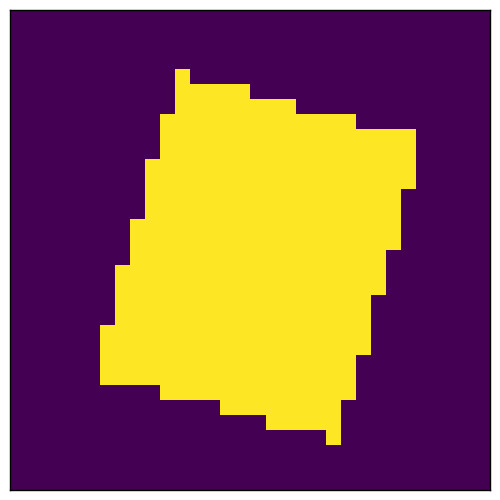
\includegraphics[width=2cm]{data/2d/distance_transform/0}
  \end{subfigure}
  \begin{subfigure}[t]{0.12\textwidth}
    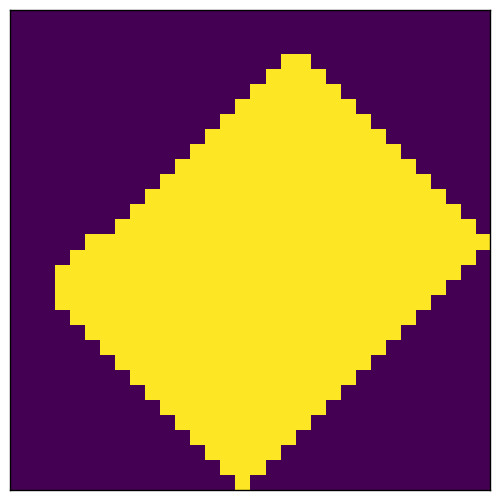
\includegraphics[width=2cm]{data/2d/distance_transform/1}
  \end{subfigure}\hspace{0.5cm}
  \begin{subfigure}[t]{0.12\textwidth}
    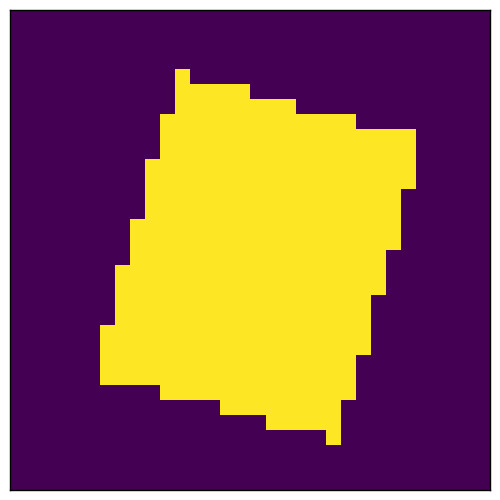
\includegraphics[width=2cm]{data/2d/distance_transform/0}
  \end{subfigure}
  \begin{subfigure}[t]{0.12\textwidth}
    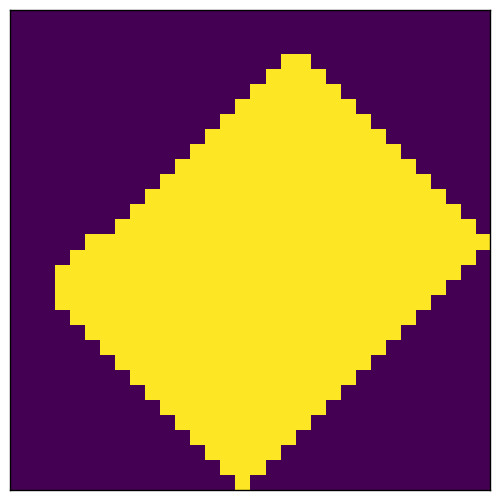
\includegraphics[width=2cm]{data/2d/distance_transform/1}
  \end{subfigure}\hspace{0.5cm}
  \begin{subfigure}[t]{0.12\textwidth}
    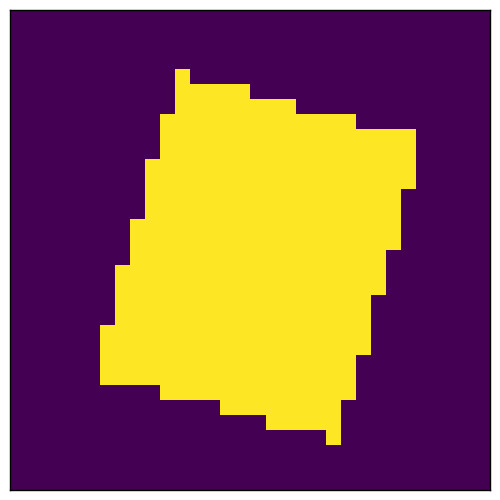
\includegraphics[width=2cm]{data/2d/distance_transform/0}
  \end{subfigure}
  \begin{subfigure}[t]{0.12\textwidth}
    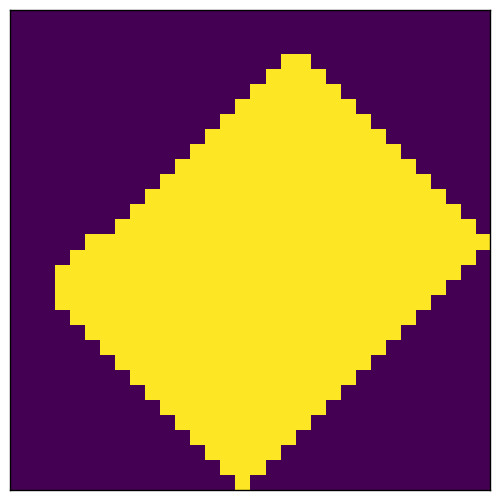
\includegraphics[width=2cm]{data/2d/distance_transform/1}
  \end{subfigure}\\
  
  \begin{subfigure}[t]{0.12\textwidth}
    \includegraphics[width=2cm]{data/2d/distance_transform/3/0_true}
  \end{subfigure}
  \begin{subfigure}[t]{0.12\textwidth}
    \includegraphics[width=2cm]{data/2d/distance_transform/3/1_true}
  \end{subfigure}\hspace{0.5cm}
  \begin{subfigure}[t]{0.12\textwidth}
    \includegraphics[width=2cm]{data/2d/distance_transform/5/0_true}
  \end{subfigure}
  \begin{subfigure}[t]{0.12\textwidth}
    \includegraphics[width=2cm]{data/2d/distance_transform/5/1_true}
  \end{subfigure}\hspace{0.5cm}
  \begin{subfigure}[t]{0.12\textwidth}
    \includegraphics[width=2cm]{data/2d/distance_transform/7/0_true}
  \end{subfigure}
  \begin{subfigure}[t]{0.12\textwidth}
    \includegraphics[width=2cm]{data/2d/distance_transform/7/1_true}
  \end{subfigure}\\
  
  \begin{subfigure}[t]{0.12\textwidth}
    \includegraphics[width=2cm]{data/2d/distance_transform/3/0_appr}
  \end{subfigure}
  \begin{subfigure}[t]{0.12\textwidth}
    \includegraphics[width=2cm]{data/2d/distance_transform/3/1_appr}
  \end{subfigure}\hspace{0.5cm}
  \begin{subfigure}[t]{0.12\textwidth}
    \includegraphics[width=2cm]{data/2d/distance_transform/5/0_appr}
  \end{subfigure}
  \begin{subfigure}[t]{0.12\textwidth}
    \includegraphics[width=2cm]{data/2d/distance_transform/5/1_appr}
  \end{subfigure}\hspace{0.5cm}
  \begin{subfigure}[t]{0.12\textwidth}
    \includegraphics[width=2cm]{data/2d/distance_transform/7/0_appr}
  \end{subfigure}
  \begin{subfigure}[t]{0.12\textwidth}
    \includegraphics[width=2cm]{data/2d/distance_transform/7/1_appr}
  \end{subfigure}
  
  %\begin{subfigure}[t]{0.12\textwidth}
  %  \includegraphics[width=2cm]{data/2d/distance_transform/3/0_err}
  %\end{subfigure}
  %\begin{subfigure}[t]{0.12\textwidth}
  %  \includegraphics[width=2cm]{data/2d/distance_transform/3/1_err}
  %\end{subfigure}\hspace{0.5cm}
  %\begin{subfigure}[t]{0.12\textwidth}
  %  \includegraphics[width=2cm]{data/2d/distance_transform/5/0_err}
  %\end{subfigure}
  %\begin{subfigure}[t]{0.12\textwidth}
  %  \includegraphics[width=2cm]{data/2d/distance_transform/5/1_err}
  %\end{subfigure}\hspace{0.5cm}
  %\begin{subfigure}[t]{0.12\textwidth}
  %  \includegraphics[width=2cm]{data/2d/distance_transform/7/0_err}
  %\end{subfigure}
  %\begin{subfigure}[t]{0.12\textwidth}
  %  \includegraphics[width=2cm]{data/2d/distance_transform/7/1_err}
  %\end{subfigure}
  \begin{tikzpicture}[overlay]
    \node at (6.75,3.55) {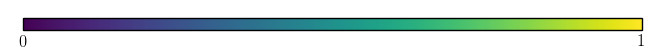
\includegraphics[height=6.5cm]{data/2d/distance_transform/colorbar}};
  \end{tikzpicture}
  
  % TODO short caption
  \caption{Illustration of the distance function approximation as discussed in
  Section \ref{sec:shape-inference-distance-function-appr} for $T = 3, 5, 7$
  iterations (from left to right). In each case, two samples are shown, including
  the original binary shape, the true distance function, the approximation and
  the error.}
  \label{fig:shape-inference-distance transform}
\end{figure}

In the ideal case, we would predict both occupancy and a signed distance functions,
avoiding the problem of having to differentiate through $\text{df}(y)$. For early
experiments, however, we decided to approximate $\text{df}(y)$ by a succession
of convolutional layers allowing to compute $\nabla_y \mathcal{L}_{\text{DL},1}$
using error backpropagation.
%The loss computation is then illustrated in Figure \ref{fig:shape-inference-point-loss}
%together with the distance function approximation.

\subsubsection{Approximate Distance Function}
\label{sec:shape-inference-distance-function-appr}

% TODO wording
The approximation relies on a simple observation: given an occupancy grid,
successive convolution with a fixed kernel $w = 1^{K \times K \times K}$ will lead to larger values
for occupied voxels and lower values for non-occupied voxels further away.
Depending on how many iterations are performed and on the size $K$ of the kernel,
far away voxels might still be $0$. Adding $1$ to every voxel, and taking the
multiplicative inverse leads to a distance function with values in $[0,1]$ that are closer to $1$
for further away voxels and closer to $0$ for occupied voxels. If we require that
the distance function is $0$ for occupied voxels, we can finally multiply by $1-y$.
In practice, we found that thresholding the predicted shape is not necessary.
An illustration of the result is given in Figure \ref{fig:shape-inference-approximation}
in terms of:

\begin{figure}
  \centering
  \begin{tikzpicture}
    \node (y) at (1.25, 0) {$y$};
    
    \node[view,minimum width=2cm,draw=black!30,text=black!50] (i) at (8.75,2.25) {$1-\cdot$};
    
    \node[conv,rotate=90,minimum width=3cm] (conv1) at (2.5,0) {$\text{conv}_{1, 1, K}$};
    \node[conv,rotate=90,minimum width=3cm] (conv2) at (3.75,0) {$\text{conv}_{1, 1, K}$};
    \node[conv,rotate=90,minimum width=3cm] (conv3) at (6.25,0) {$\text{conv}_{1, 1, K}$};
    \node[conv,rotate=90,minimum width=3cm] (conv4) at (7.5,0) {$\text{conv}_{1, 1, K}$};
    \node[view,rotate=90,minimum width=3cm] (p5) at (8.75,0) {$\cdot+1$};
    \node[view,rotate=90,minimum width=3cm] (n6) at (10,0) {$1/\cdot$};
    \node[view,rotate=90,minimum width=3cm,draw=black!40,text=black!40] (m) at (11.25,0) {$\cdot$};
    \node (dfy) at (12.75, 0) {$\tilde{\text{df}}(y)$};
    
    \draw[-,draw=black!50] (y) -- (1.25,2.25);
    \draw[->,draw=black!50] (1.25,2.25) -- (i);
    \draw[->] (y) -- (conv1);
    \draw[->] (conv1) -- (conv2);
    \draw[->,dashed] (conv2) -- (conv3);
    \draw[->] (conv3) -- (conv4);
    \draw[->] (conv4) -- (p5);
    \draw[->] (p5) -- (n6);
    \draw[->] (n6) -- (m);
    
    \draw[-,draw=black!50] (i) -- (11.25,2.25);
    \draw[->,draw=black!50](11.25,2.25) -- (m);
    
    \draw[->] (m) -- (dfy);
  \end{tikzpicture}
  \vskip 6px
  % TODO short caption
  \caption{Illustration of the layers required to approximate the distance function
  of an occupancy grid given the occupancy probabilities $y$. The intuition is
  also described in the text. The gray path illustrates the alternative variant
  where we ensure that the approximated distance function is $0$
  at occupied voxels.}
  \label{fig:shape-inference-approximation}
\end{figure}

%\begin{definition}
%  A threshold layer $\text{thr}_\tau$ takes as input a tensor
%  $x \in \mathbb{R}^{B \times C \times H \times D \times W}$
%  and computes
%  \begin{align}
%   (\text{thr}_\tau(x))_i = \begin{cases}1&\quad x_i \geq \tau\\0&\quad x_i < \tau\end{cases}.
%  \end{align}
%\end{definition}

\begin{definition}
  Let $\times$ be an element-wise tensor operation,
  $x$ an arbitrary input tensor and $s$ be a fixed tensor, then
  the corresponding layers $\cdot \times s$ or $s \times \cdot$
  compute
  \begin{align}
    ((\cdot \times s)(x))_i = x_i \times s_i\\
    ((s_i \times \cdot)(x))_i = s_i \times x_i.
  \end{align}
  These layers can analogously be extended to cases
  taking two tensors as input.
\end{definition}

\subsection{Practical Considerations}

When using a variational auto-encoder prior, the decoder, \ie $p(y|z)$ is
retained and only the encoder is trained. In the case of a
probabilistic PCA prior, we use
\begin{align}
  \theta(z) = g(Uz + \mu)
\end{align}
as decoder, where $g$ is a clipping function or a scaled sigmoid.
This can be implemented as fully-connected layer with bias and non-linearity.
